\documentclass[conference]{IEEEtran}
\usepackage[utf8]{inputenc}
\usepackage[T1]{fontenc}
\usepackage[spanish,es-tabla]{babel}
\usepackage{amsmath,amssymb,amsfonts}
\usepackage{graphicx}
\usepackage{textcomp}
\usepackage{xcolor}
\usepackage{booktabs}
\usepackage{cite}
\usepackage{url}
\usepackage{microtype}
\usepackage{tabularx}

\begin{document}

\title{Pronóstico de Demanda Eléctrica Horaria mediante una Arquitectura Híbrida Convolucional-Recurrente (CNN-LSTM): Estudio Comparativo sobre la Red PJM\\
\large Entregable 2: Métodos y Resultados Preliminares}

\author{
    \IEEEauthorblockN{Juan José Villalba}
    \IEEEauthorblockA{\textit{Facultad de Ingeniería y Ciencias Aplicadas} \\
    \textit{Universidad de las Américas}\\
    Quito, Ecuador \\
    juan.villalba@udla.edu.ec}
    \and
    \IEEEauthorblockN{Sebastián Cadena}
    \IEEEauthorblockA{\textit{Facultad de Ingeniería y Ciencias Aplicadas} \\
    \textit{Universidad de las Américas}\\
    Quito, Ecuador \\
    sebastian.cadena@udla.edu.ec}
    \and
    \IEEEauthorblockN{Anthonny Mosquera}
    \IEEEauthorblockA{\textit{Facultad de Ingeniería y Ciencias Aplicadas} \\
    \textit{Universidad de las Américas}\\
    Quito, Ecuador \\
    anthonny.mosquera@udla.edu.ec}
}

\maketitle

\begin{abstract}
El pronóstico preciso de demanda eléctrica horaria en horizontes de 24 horas (\textit{Day-Ahead}) es esencial para la estabilidad de las redes inteligentes, la programación económica de despacho térmico y el aprovechamiento de generación renovable variable. Sin embargo, las series eléctricas regionales exhiben estacionalidad multiescala combinada con perturbaciones no lineales difíciles de modelar mediante enfoques estadísticos lineales o redes recurrentes homogéneas sin extracción local de patrones. Este segundo entregable evolutivo presenta la implementación reproducible completa y los resultados preliminares del modelo híbrido convolucional-recurrente (\textbf{CNN1D-LSTM}) sobre el registro histórico real de la zona oriental de PJM Interconnection (\textit{PJME}, 2002--2018). Bajo una partición cronológica estricta (70\,\% entrenamiento, 15\,\% validación y 15\,\% prueba ciega sellada hasta la entrega final), limpieza causal de transiciones de horario de verano (DST) y verificación automatizada contra fuga de datos, se contrasta la arquitectura propuesta frente a cuatro líneas base: Persistencia 24\,h, Persistencia 168\,h, Perfil Horario Condicional, \textit{SARIMA}$(1,1,1)\times(1,1,1)_{24}$ y una red \textbf{LSTM Pura} arquitectónicamente equivalente. En el conjunto completo de validación (21{,}545 ventanas de 24\,h; tres semillas aleatorias), \textbf{CNN1D-LSTM} alcanza un RMSE promedio de $1{,}834.00 \pm 38.41$\,MW ($\text{MAPE}=4.24\%$, $R^2=0.9121$) con latencia de $0.0131$\,ms por muestra, superando a Persistencia 24\,h ($3{,}062.79$\,MW), a LSTM Pura ($1{,}872.38 \pm 33.68$\,MW) y reduciendo el RMSE en $29.1\,\%$ respecto a SARIMA sobre 28 días estacionales estratificados ($1{,}608.88$ vs.\ $2{,}269.12$\,MW). Asimismo, el análisis desagregado por regímenes críticos evidencia un suavizado leve en el decil extremo superior ($\ge P_{90}$) asociado a la ausencia de variables climáticas exógenas y al submuestreo temporal, orientando los estudios de ablación y optimización de las últimas cinco semanas.
\end{abstract}

\begin{IEEEkeywords}
Pronóstico de carga eléctrica, CNN1D-LSTM, SARIMA, series temporales multihito, redes inteligentes, PJM Interconnection.
\end{IEEEkeywords}

\section{Introducción}

La operación confiable de los sistemas modernos de potencia requiere equilibrar continuamente la generación despachada y el consumo eléctrico en tiempo real. Errores sistemáticos por subestimación comprometen los márgenes de seguridad térmica de líneas de transmisión, mientras que la sobreestimación incrementa el consumo de combustible y las emisiones asociadas al mantenimiento de reserva rodante innecesaria \cite{hippert2001neural,taylor2003short}. En mercados eléctricos de esquema \textit{Day-Ahead}, la tarea crítica consiste en proyectar simultáneamente la curva horaria completa de las próximas 24 horas (\textit{Short-Term Load Forecasting}, STLF) frente a estacionalidad jerárquica superpuesta (diaria, semanal y anual) y choques no lineales derivados de olas de calor o frentes fríos \cite{lim2021time,ahajjam2022experimental}.

\subsection{Trabajo Relacionado y Brecha Investigativa}
La literatura sobre STLF abarca desde formulaciones estadísticas clásicas hasta arquitecturas profundas híbridas. Los modelos autorregresivos estacionales (\textit{SARIMA}) y de suavizado exponencial doble estacional \cite{taylor2003short} ofrecen alta interpretabilidad estadística, pero su naturaleza lineal y costo cúbico de estimación dificultan capturar transiciones no lineales abruptas sobre series históricas de gran escala \cite{hippert2001neural}. Con el auge del aprendizaje profundo, Shi et al.\ \cite{shi2018deep} y Kong et al.\ \cite{kong2019short} demostraron que las redes de memoria a largo plazo (LSTM) \cite{hochreiter1997long} superan a los modelos lineales al modelar dependencias temporales complejas, aunque el entrenamiento directo sobre secuencias crudas incrementa la latencia secuencial y muestra sensibilidad al ruido de alta frecuencia \cite{ageng2021short}.

Para mitigar estas limitaciones, diversas investigaciones han acoplado extractores convolucionales unidimensionales (CNN-1D) antes de etapas recurrentes. Kim y Cho \cite{kim2019predicting} mostraron mejoras consistentes con CNN-LSTM en consumo residencial, mientras Alhussein et al.\ \cite{alhussein2020hybrid} y Sajjad et al.\ \cite{sajjad2020novel} reportaron ganancias frente a LSTM y GRU puras al reducir la carga secuencial mediante filtros locales. De modo similar, Sadaei et al.\ \cite{sadaei2019short} combinaron CNN-1D con lógica difusa en redes regionales, Rafi et al.\ \cite{rafi2021short} integraron CNN-LSTM para horizontes multihito, y Alsharekh et al.\ \cite{alsharekh2022improving} validaron arquitecturas residuales R-CNN con ML-LSTM sobre datos de la red PJM. No obstante, persisten brechas relevantes en la reproducibilidad comparativa: muchos estudios omiten una verificación unitaria estricta contra fuga de datos (\textit{data leakage}) \cite{lim2021time}, comparan modelos heterogéneos sin igualar la capacidad de la cabeza recurrente o evalúan únicamente métricas agregadas sin desagregar el desempeño en horas pico críticas ni el costo de inferencia. La Tabla~\ref{tab:estado_arte} sintetiza este contraste.

\begin{table*}[t]
\centering
\caption{Síntesis Crítica de Literatura Relacionada Frente a la Implementación Actual}
\label{tab:estado_arte}
\footnotesize
\begin{tabularx}{\textwidth}{l p{2.9cm} p{2.6cm} p{2.3cm} p{4.6cm}}
\toprule
\textbf{Referencia} & \textbf{Arquitectura / Método} & \textbf{Dominio / Datos} & \textbf{Horizonte} & \textbf{Brecha Abordada en Nuestro Trabajo} \\
\midrule
Taylor \cite{taylor2003short} & Suavizado / ARIMA estac. & Demanda nacional & 1--24\,h & Supuestos lineales; degradación en picos climáticos. \\
Shi et al.\ \cite{shi2018deep} & Pooling Deep RNN & Hogares (smart meters) & 1 paso / Horario & Sin extracción convolucional; escala residencial. \\
Kong et al.\ \cite{kong2019short} & LSTM secuencial & Residencial individual & Horario & Alto ruido estocástico; no evalúa latencia multihito. \\
Kim \& Cho \cite{kim2019predicting} & CNN-LSTM & Consumo residencial & Horario / Diario & Sin análisis de ablación en red de transmisión regional. \\
Sadaei et al.\ \cite{sadaei2019short} & CNN-1D + Series difusas & Red eléctrica regional & 24\,h / Horario & Reglas difusas heurísticas de difícil reproducibilidad. \\
Alhussein et al.\ \cite{alhussein2020hybrid} & CNN-1D + LSTM & Carga agregada / ind. & Horario & Sin codificación cíclica trigonométrica explícita. \\
Sajjad et al.\ \cite{sajjad2020novel} & CNN-1D + GRU & Residencial agregada & 1--12\,h & No evalúa paridad controlada vs.\ LSTM pura a 24\,h. \\
Rafi et al.\ \cite{rafi2021short} & CNN + LSTM integrada & Demanda eléctrica & Multihito & Sin auditoría automatizada anti-fuga ni latencia GPU. \\
Alsharekh et al.\ \cite{alsharekh2022improving} & R-CNN + ML-LSTM & PJM / Comercial & Multihito & Mayor complejidad residual; sin contraste con SARIMA. \\
\midrule
\textbf{Este Trabajo} & \textbf{CNN1D-LSTM vs.\ Paridad} & \textbf{PJM East (145{,}392\,h)} & \textbf{24\,h multihito} & \textbf{Paridad LSTM, tests anti-leakage, val/test sellado y latencia.} \\
\bottomrule
\end{tabularx}
\end{table*}

\subsection{Preguntas de Investigación y Alcance de la Entrega}
En continuidad con la propuesta aprobada del Entregable 1 (incorporando mayor rigor en la especificación reproducible y una revisión bibliográfica ampliada), el estudio responde dos preguntas centrales:
\begin{itemize}
    \item \textbf{PI-1:} ¿En qué magnitud la arquitectura híbrida CNN1D-LSTM supera a líneas base estadísticas (SARIMA y heurísticas) y a una LSTM Pura con idéntico bloque recurrente sobre horizonte de 24\,h en PJME?
    \item \textbf{PI-2:} ¿Cómo influye la extracción convolucional local en el error por horizonte ($h=1\dots 24$) y en regímenes críticos (horas pico $14\text{--}20\,\text{h}$, decil $\ge P_{90}$ y fines de semana)?
\end{itemize}
Con el fin de preservar la integridad experimental hacia el artículo final (Entregable 3), todos los resultados preliminares aquí reportados se evalúan exclusivamente sobre el conjunto de \textbf{validación}, manteniendo el conjunto de \textbf{prueba ciega} completamente sellado.

\section{Métodos}

\subsection{Conjunto de Datos, Limpieza Causal y Partición}
Se emplea el registro horario real de consumo eléctrico de \textit{PJM Interconnection LLC} para la zona oriental (\textit{PJME}) \cite{pjm2018data}, compuesto por 145{,}366 mediciones originales entre el 1 de enero de 2002 (01:00) y el 3 de agosto de 2018 (00:00). Para garantizar continuidad física sin introducir información futura (\textit{lookahead bias}), el pipeline aplica: (1) ordenamiento cronológico estricto; (2) resolución determinista de marcas de tiempo duplicadas debidas al retroceso horario de otoño (\textit{Daylight Saving Time}, DST) mediante promedio horario; (3) reindexación a malla horaria continua (\texttt{freq="h"}) e interpolación lineal acotada sobre los huecos aislados del adelanto DST de primavera. La Tabla~\ref{tab:data_audit} resume la auditoría exacta del conjunto limpio (145{,}392 horas, brecha consecutiva máxima de solo 1 hora).

\begin{table}[htbp]
\centering
\caption{Auditoría de Limpieza DST y Partición Cronológica (PJME Real)}
\label{tab:data_audit}
\footnotesize
\begin{tabularx}{\columnwidth}{l l r}
\toprule
\textbf{Concepto / Partición} & \textbf{Rango Temporal / Detalle} & \textbf{Valor} \\
\midrule
Registros crudos iniciales & 2002-01-01 01:00 -- 2018-08-03 00:00 & 145{,}366 \\
Duplicados DST resueltos & Promedio determinista de hora repetida & 4 \\
Horas faltantes imputadas & Interpolación lineal (hueco máx. = 1\,h) & 30 \\
Serie horaria limpia total & Media $32{,}078.9$\,MW ($\sigma=6{,}464.3$\,MW) & 145{,}392 \\
\midrule
Entrenamiento (\texttt{train}, 70\,\%) & 2002-01-01 01:00 -- 2013-08-11 14:00 & 101{,}774 \\
Validación (\texttt{val}, 15\,\%) & 2013-08-11 15:00 -- 2016-02-06 06:00 & 21{,}808 \\
Prueba ciega (\texttt{test}, 15\,\%) & 2016-02-06 07:00 -- 2018-08-03 00:00 & 21{,}810 \\
\midrule
Ventanas \texttt{train} / \texttt{val} / \texttt{test} & Tensores $W=72 \to H=24$ aislados & 101{,}511 / 21{,}545 / 21{,}547 \\
Umbral pico $P_{90}$ (\texttt{train}) & Percentil 90 solo de entrenamiento & 40{,}850.7\,MW \\
\bottomrule
\end{tabularx}
\end{table}

\subsection{Ingeniería de Características y Prevención de Fuga de Datos}
Cada partición (\texttt{train}, \texttt{val}, \texttt{test}) se procesa de manera \textbf{aislada} tras el corte temporal para impedir cruces de frontera en las ventanas deslizantes. Dentro de cada partición se construyen $F=9$ canales causales: la demanda horaria (\texttt{PJME\_MW}), su retardo semanal estricto de 7 días (\texttt{lag\_168} $= y_{t-168}$), el indicador binario de fin de semana (\texttt{is\_weekend}) y la codificación trigonométrica continua para hora del día ($T=24$), día de la semana ($T=7$) y mes ($T=12$):
\begin{equation}
    x_{\sin}^{(T)}(t) = \sin\!\left(\frac{2\pi t}{T}\right), \qquad x_{\cos}^{(T)}(t) = \cos\!\left(\frac{2\pi t}{T}\right).
\end{equation}
Las variables de carga (\texttt{PJME\_MW} y \texttt{lag\_168}) se escalan al intervalo $[0,1]$ mediante transformación Min-Max ajustada \textbf{exclusivamente} sobre \texttt{train}:
\begin{equation}
    z_t = \frac{y_t - \min(Y_{\text{train}})}{\max(Y_{\text{train}}) - \min(Y_{\text{train}})},
\end{equation}
donde $\min(Y_{\text{train}})=14{,}544.0$\,MW y $\max(Y_{\text{train}})=62{,}009.0$\,MW. Las entradas se estructuran como tensores $\mathbf{X} \in \mathbb{R}^{B \times W \times F}$ con ventana histórica $W=72$\,h para predecir simultáneamente el vector objetivo $\hat{\mathbf{y}} \in \mathbb{R}^{B \times H}$ con $H=24$\,h ($t+1 \dots t+24$). Una suite automatizada de 6 pruebas unitarias en \texttt{pytest} (\texttt{tests/test\_data\_leakage.py} y \texttt{tests/test\_models.py}) valida la monotonía temporal, la limpieza DST, el aislamiento de splits y que el escalador nunca observe datos de validación o prueba.

\subsection{Arquitecturas Neuronales bajo Paridad Controlada}
Con el propósito de aislar el efecto neto de la etapa convolucional (\textbf{PI-1} y \textbf{PI-2}), la línea base profunda (\textbf{LSTM Pura}) y el modelo propuesto (\textbf{CNN1D-LSTM}) comparten exactamente la misma etapa recurrente y cabeza de proyección (\texttt{RecurrentForecastHead}), como ilustra la Fig.~\ref{fig:arch}.

\begin{figure*}[t]
    \centering
    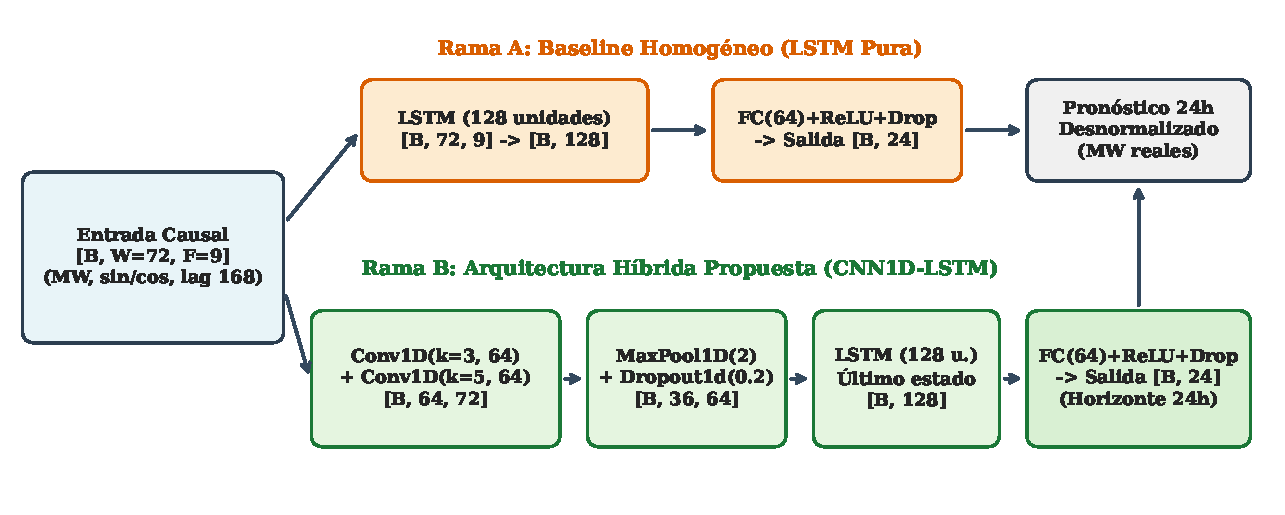
\includegraphics[width=0.86\textwidth]{figures/fig2_architecture_diagram.pdf}
    \caption{Diseño experimental controlado entre la línea base LSTM Pura (Rama A) y la arquitectura híbrida propuesta CNN1D-LSTM (Rama B), compartiendo idéntica capacidad recurrente y cabeza densa de 24 salidas.}
    \label{fig:arch}
\end{figure*}

\begin{itemize}
    \item \textbf{LSTM Pura (80{,}984 parámetros):} Recibe directamente $\mathbf{X} \in \mathbb{R}^{B \times 72 \times 9}$ en una capa LSTM de 128 unidades ocultas; su último estado $\mathbf{h}_T \in \mathbb{R}^{128}$ pasa por una capa densa de 64 neuronas (ReLU, Dropout 0.2) hacia la salida lineal de 24 horas.
    \item \textbf{CNN1D-LSTM (131{,}480 parámetros):} Transpone la entrada a $\mathbb{R}^{B \times 9 \times 72}$ y aplica dos convoluciones unidimensionales con 64 filtros cada una (núcleos $k_1=3$ y $k_2=5$, \textit{padding} simétrico causal dentro de la ventana histórica y activación ReLU):
    \begin{equation}
        \mathbf{C}_j = \mathrm{ReLU}\!\left(\sum_{i=1}^{F} \mathbf{X}_i * \mathbf{K}_{i,j} + b_j\right),
    \end{equation}
    seguidas de \texttt{MaxPool1D(2)} (reduciendo la secuencia temporal $72 \to 36$) y regularización espacial \texttt{Dropout1d(0.2)} sobre mapas de características antes de alimentar la misma capa LSTM de 128 unidades y proyección densa $64 \to 24$.
\end{itemize}

\subsection{Líneas Base Estadísticas y Heurísticas}
Todas las líneas base se evalúan sobre las \textbf{mismas ventanas y en MW reales desnormalizados}:
\begin{enumerate}
    \item \textbf{Persistencia 24\,h:} $\hat{y}_{t+h} = y_{t+h-24}$ ($h=1\dots 24$).
    \item \textbf{Persistencia 168\,h:} $\hat{y}_{t+h} = y_{t+h-168}$ (misma hora de la semana previa).
    \item \textbf{Perfil Horario Condicional:} Promedio histórico en \texttt{train} condicionado por par $(\text{fin de semana}, \text{hora})$.
    \item \textbf{SARIMA$(1,1,1)\times(1,1,1)_{24}$:} Justificado mediante pruebas formales sobre el último año de \texttt{train} ($n=8{,}760$\,h): la serie original exhibe no estacionariedad de nivel según KPSS ($\text{stat}=1.663$, $p \le 0.01$; ADF $=-6.048$, $p=1.30\times 10^{-7}$), mientras la diferenciación estacional $(1-B^{24})y_t$ alcanza estacionariedad robusta ($\text{ADF}=-11.657$, $p=1.98\times 10^{-21}$). Debido al alto costo computacional de estimar modelos de espacio de estados sobre $>10^5$ horas, SARIMA se evalúa de forma causal sobre 28 orígenes diarios estratificados (\texttt{00:00}--\texttt{23:00}) distribuidos uniformemente en \texttt{val}, ajustando cada modelo sobre los 60 días previos ($1{,}440$\,h) y comparando en ese mismo subconjunto (672\,h) a todos los modelos.
\end{enumerate}

\subsection{Entorno, Hiperparámetros y Métricas de Evaluación}
La implementación se desarrolló en Python 3.13.5, PyTorch 2.11.0+cu128 y \texttt{statsmodels} 0.15.0 sobre una GPU NVIDIA GeForce RTX 3050 (6\,GB VRAM). Los modelos neuronales se entrenaron minimizando el Error Cuadrático Medio (MSE) con el optimizador Adam ($\alpha=10^{-3}$, \textit{weight decay} $=10^{-5}$, recorte de gradiente $\Vert g \Vert_2 \le 1.0$, tamaño de lote $B=128$, máximo 50 épocas), planificador \texttt{ReduceLROnPlateau} (factor 0.5, paciencia 3) y \texttt{EarlyStopping} (paciencia 8). Cada arquitectura se entrenó con \textbf{tres semillas} ($\{42, 123, 456\}$) reportando media $\pm$ desviación estándar.

Tras invertir el escalado a MW reales, se evalúan RMSE, MAE, MAPE (\%) y $R^2$ de forma global, por paso de horizonte $h=1\dots 24$, por régimen operativo (pico $\ge P_{90}=40{,}850.7$\,MW, franja operativa $14\text{--}20\,\text{h}$, días laborales vs.\ fines de semana) y latencia de inferencia sincronizada en GPU (ms/ventana).

\section{Resultados Preliminares}

\subsection{Análisis Exploratorio y Validación de Estacionalidad}
La Fig.~\ref{fig:eda} resume los patrones estructurales de la red PJME. Se distingue claramente la periodicidad anual bimodal (picos de verano por climatización de hasta $62{,}009$\,MW y picos invernales secundarios), la reducción sistemática de carga los fines de semana junto a su doble cresta diurna, y la fuerte autocorrelación en los múltiplos de $24\,\text{h}$, $72\,\text{h}$ y $168\,\text{h}$ ($\text{ACF}>0.70$), respaldando empíricamente la ventana $W=72$ y la inclusión de \texttt{lag\_168}.

\begin{figure*}[t]
    \centering
    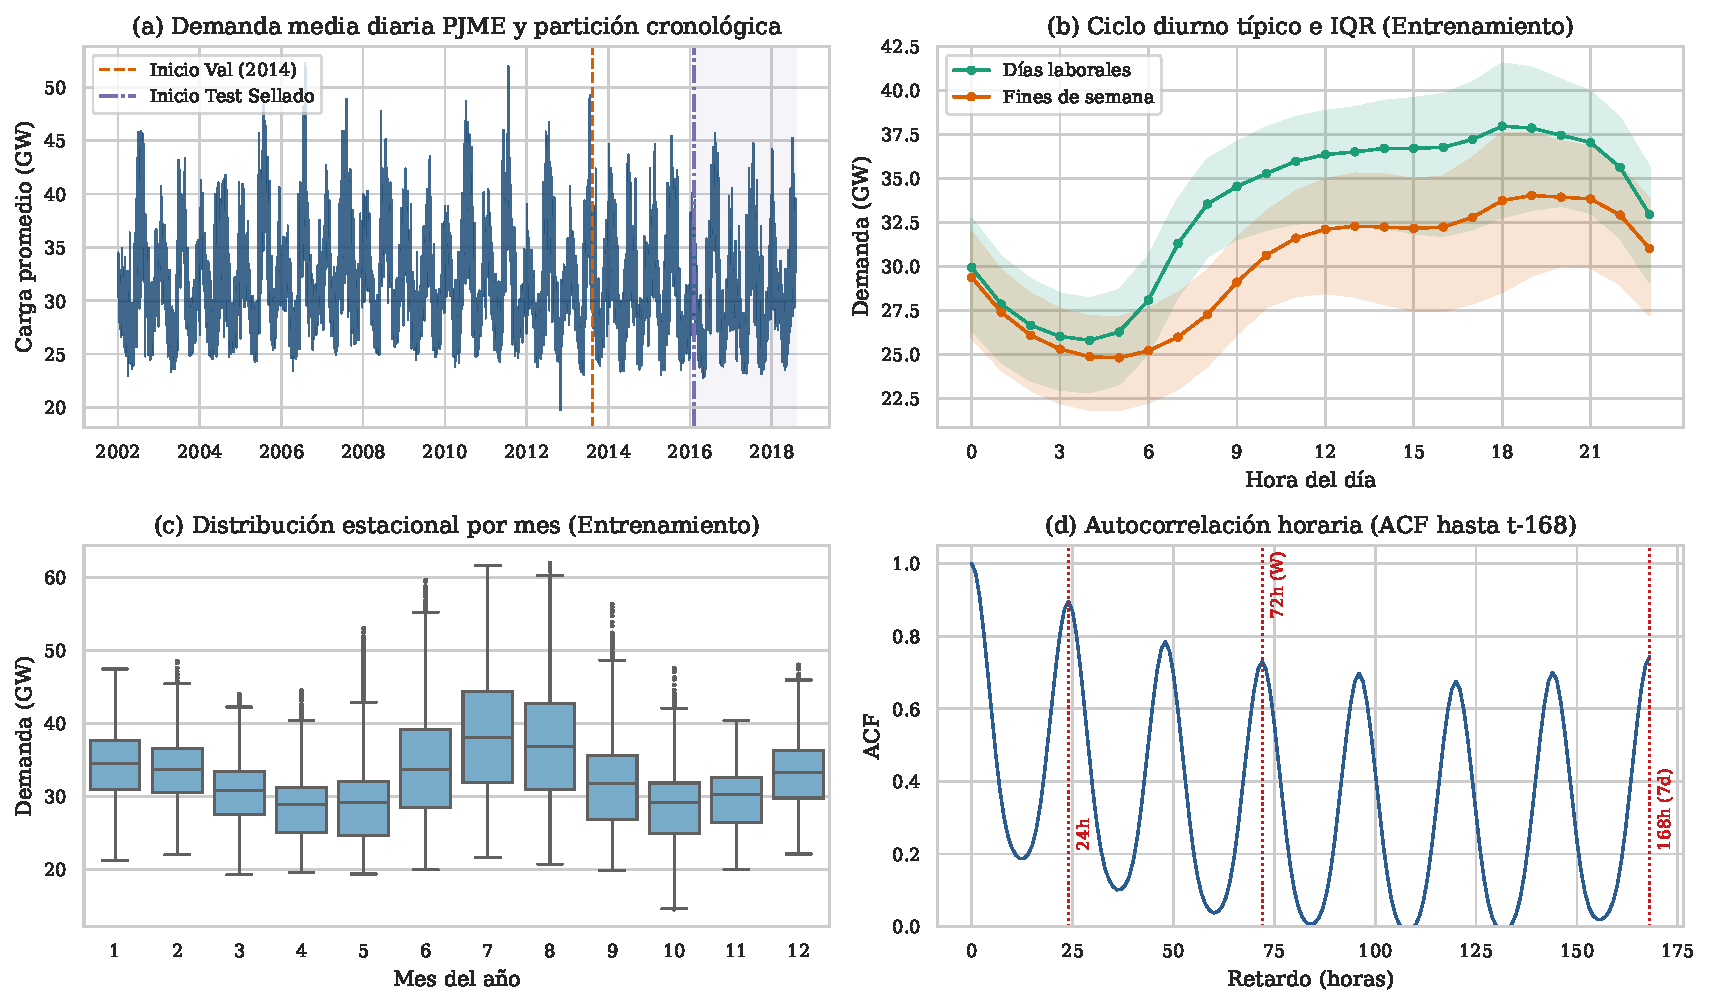
\includegraphics[width=0.88\textwidth]{figures/fig1_eda_pjme.pdf}
    \caption{Análisis exploratorio del registro real PJME (2002--2018): (a) demanda media diaria con particiones cronológicas; (b) ciclo diurno e IQR laboral vs.\ fin de semana; (c) distribución mensual estacional; (d) autocorrelación horaria hasta 168\,h.}
    \label{fig:eda}
\end{figure*}

\subsection{Convergencia y Desempeño Comparativo en Validación}
La Fig.~\ref{fig:curves} muestra las curvas de entrenamiento y validación para las tres semillas de ambos modelos neuronales. La convergencia resulta estable sin divergencias de gradiente ni sobreajuste severo; la pérdida de validación se estabiliza en torno a $1.45\text{--}1.62 \times 10^{-3}$, siendo ligeramente menor que la de entrenamiento debido al efecto de \texttt{Dropout} activo únicamente en entrenamiento y a la mayor varianza de picos históricos en el periodo 2002--2013. \textbf{CNN1D-LSTM} alcanza su mínimo global en la semilla 42 ($\text{val\_mse}=0.001448$, época 39) frente al mejor registro de \textbf{LSTM Pura} ($\text{val\_mse}=0.001512$, semilla 123, época 42).

\begin{figure*}[t]
    \centering
    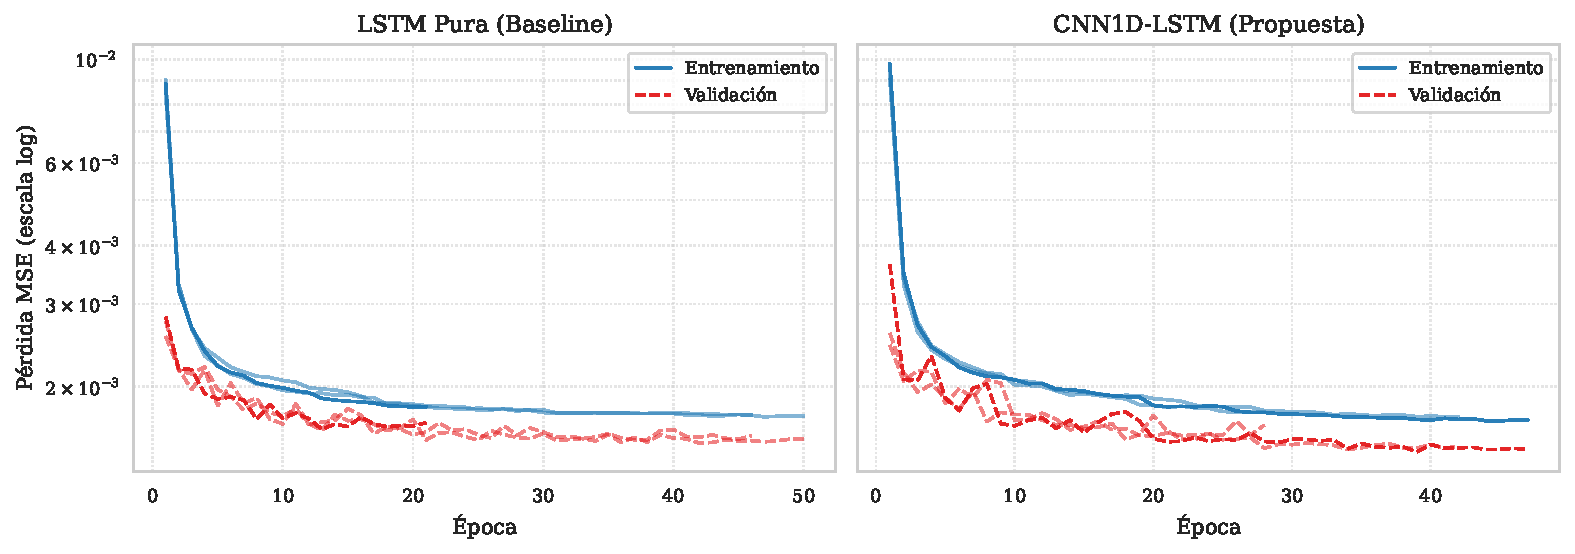
\includegraphics[width=0.84\textwidth]{figures/fig3_training_curves.pdf}
    \caption{Curvas de pérdida MSE (escala logarítmica) durante entrenamiento y validación en GPU RTX 3050 a través de las tres semillas aleatorias ($\{42, 123, 456\}$).}
    \label{fig:curves}
\end{figure*}

La Tabla~\ref{tab:full_val} consolida el desempeño sobre el \textbf{100\,\% de las ventanas de validación} ($21{,}545$ ventanas; $517{,}080$ predicciones horarias). Ambas arquitecturas profundas reducen drásticamente el error frente a las líneas base heurísticas: respecto a Persistencia 24\,h ($\text{RMSE}=3{,}062.79$\,MW, $\text{MAPE}=7.01\%$), \textbf{CNN1D-LSTM} reduce el RMSE en \textbf{40.1\,\%} ($1{,}834.00 \pm 38.41$\,MW) y mejora a \textbf{LSTM Pura} ($1{,}872.38 \pm 33.68$\,MW) en RMSE, MAE, MAPE y $R^2$. Un resultado destacable es la \textbf{latencia de inferencia}: a pesar de contar con 62\,\% más parámetros ($131{,}480$ vs.\ $80{,}984$), \textbf{CNN1D-LSTM} infiere más rápido por ventana ($0.0131$\,ms vs.\ $0.0156$\,ms en GPU) debido a que el \texttt{MaxPool1D(2)} reduce a la mitad el número de pasos procesados secuencialmente por la celda LSTM.

\begin{table*}[t]
\centering
\caption{Desempeño Comparativo Global en Validación Completa (2013--2016; 21{,}545 Ventanas de 24\,h)}
\label{tab:full_val}
\footnotesize
\begin{tabular}{l c c c c r r r}
\toprule
\textbf{Modelo} & \textbf{RMSE (MW)} & \textbf{MAE (MW)} & \textbf{MAPE (\%)} & $\mathbf{R^2}$ & \textbf{Parám.} & \textbf{Entren. (s)} & \textbf{Infer. (ms/muestra)} \\
\midrule
Perfil Condicional & $4{,}926.99$ & $4{,}082.54$ & $13.23$ & $0.3660$ & 0 & --- & --- \\
Persistencia 168\,h & $4{,}278.03$ & $3{,}161.38$ & $9.78$ & $0.5220$ & 0 & --- & --- \\
Persistencia 24\,h & $3{,}062.79$ & $2{,}240.53$ & $7.01$ & $0.7550$ & 0 & --- & --- \\
LSTM Pura (3 seeds) & $1{,}872.38 \pm 33.68$ & $1{,}375.92 \pm 30.81$ & $4.36 \pm 0.10$ & $0.9084 \pm 0.0033$ & $80{,}984$ & $179.4$ & $0.0156$ \\
\textbf{CNN1D-LSTM (3 seeds)} & $\mathbf{1{,}834.00 \pm 38.41}$ & $\mathbf{1{,}340.91 \pm 49.11}$ & $\mathbf{4.24 \pm 0.18}$ & $\mathbf{0.9121 \pm 0.0037}$ & $131{,}480$ & $213.7$ & $\mathbf{0.0131}$ \\
\bottomrule
\end{tabular}
\end{table*}

La Tabla~\ref{tab:sarima_matched} presenta la comparación emparejada frente a \textbf{SARIMA$(1,1,1)\times(1,1,1)_{24}$} sobre los 28 días estratificados ($672$\,h). SARIMA supera claramente a las heurísticas ($\text{RMSE}=2{,}269.12$\,MW, $\text{MAPE}=5.17\%$), pero requiere $10.11$\,s promedio de ajuste por origen ($283.21$\,s totales; AIC medio $19{,}744.6$) y es ampliamente superado por LSTM Pura ($1{,}689.39$\,MW) y por \textbf{CNN1D-LSTM} ($\mathbf{1{,}608.88}$\,MW, $\text{MAPE}=3.72\%$, $R^2=0.9316$, una reducción de \textbf{29.1\,\%} en RMSE frente a SARIMA).

\begin{table}[htbp]
\centering
\caption{Comparativa Emparejada con SARIMA (28 Días Estratificados en Validación)}
\label{tab:sarima_matched}
\footnotesize
\begin{tabular}{l c c c c}
\toprule
\textbf{Modelo} & \textbf{RMSE (MW)} & \textbf{MAE (MW)} & \textbf{MAPE (\%)} & $\mathbf{R^2}$ \\
\midrule
Perfil Condicional & $5{,}063.10$ & $4{,}053.41$ & $13.07$ & $0.3222$ \\
Persistencia 168\,h & $3{,}882.30$ & $2{,}909.22$ & $8.77$ & $0.6015$ \\
Persistencia 24\,h & $3{,}078.51$ & $2{,}324.74$ & $7.21$ & $0.7494$ \\
SARIMA$(1,1,1)\times(1,1,1)_{24}$ & $2{,}269.12$ & $1{,}665.04$ & $5.17$ & $0.8639$ \\
LSTM Pura & $1{,}689.39$ & $1{,}260.35$ & $3.94$ & $0.9245$ \\
\textbf{CNN1D-LSTM} & $\mathbf{1{,}608.88}$ & $\mathbf{1{,}191.85}$ & $\mathbf{3.72}$ & $\mathbf{0.9316}$ \\
\bottomrule
\end{tabular}
\end{table}

\subsection{Análisis por Horizonte y Regímenes Operativos (PI-2)}
La Fig.~\ref{fig:forecasts} ilustra el comportamiento cualitativo sobre siete días consecutivos y sobre el episodio pico máximo de la muestra estratificada (20 de julio de 2015, $\sim 55$\,GW). Mientras SARIMA subestima el máximo veraniego en cerca de 3\,GW (proyectando $\sim 52$\,GW), ambos modelos neuronales capturan con fidelidad la amplitud y fase de la cresta diaria, aunque en jornadas con cambios bruscos de carga interdiaria (17 y 19 de junio) exhiben desviaciones de amplitud compartidas.

\begin{figure*}[t]
    \centering
    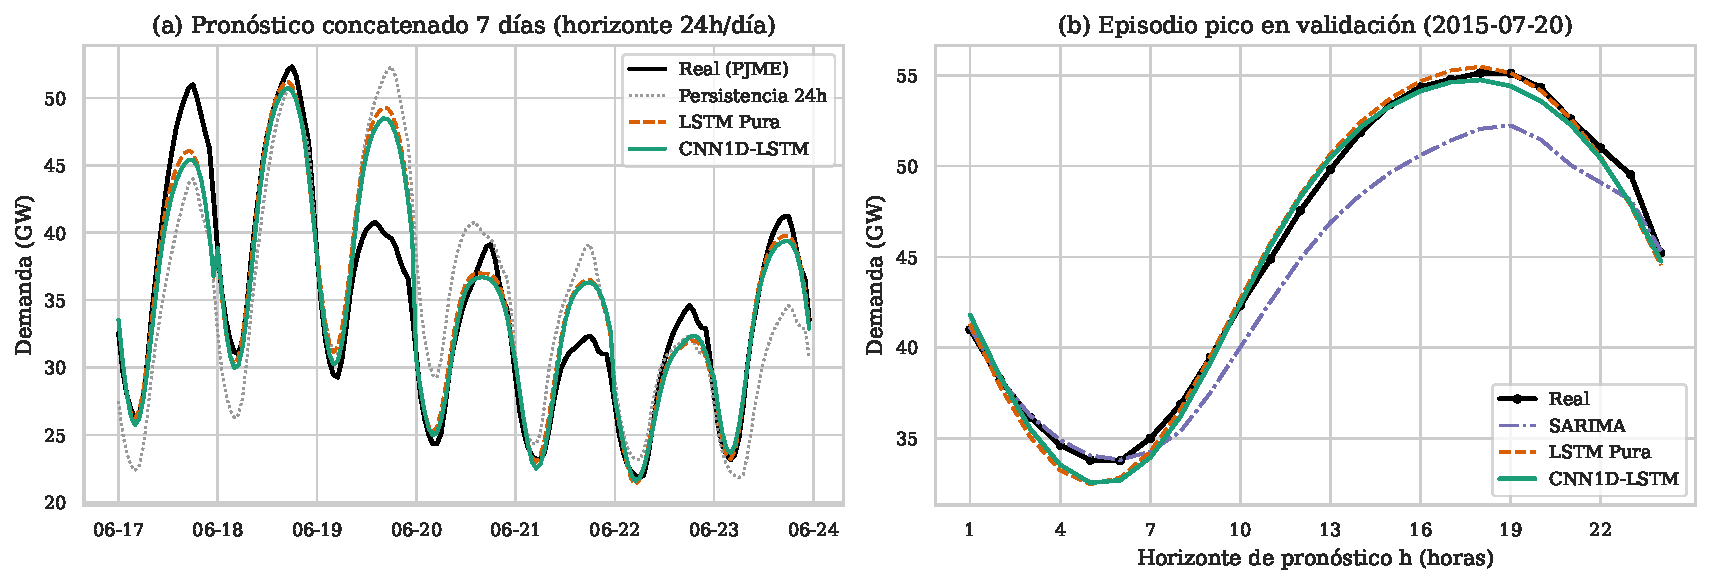
\includegraphics[width=0.88\textwidth]{figures/fig4_forecast_comparison.pdf}
    \caption{Comparación visual de pronósticos en validación: (a) trayectoria concatenada de 7 días consecutivos; (b) episodio de demanda pico estival del 20 de julio de 2015 frente a SARIMA.}
    \label{fig:forecasts}
\end{figure*}

La Fig.~\ref{fig:horizon_regimes} y la Tabla~\ref{tab:regimes} desagregan el desempeño del mejor modelo de cada familia por horizonte $h=1\dots 24$ y régimen operativo. \textbf{CNN1D-LSTM} mantiene consistentemente menor RMSE que \textbf{LSTM Pura} entre las horas $h=2$ y $h=24$ ($850.8 \to 2{,}314.8$\,MW vs.\ $826.2 \to 2{,}330.7$\,MW), así como en la franja pico diurna de $14\text{--}20\,\text{h}$ ($2{,}108.24$ vs.\ $2{,}138.31$\,MW), en días laborales ($1{,}861.49$ vs.\ $1{,}907.66$\,MW) y en fines de semana ($1{,}660.51$ vs.\ $1{,}680.61$\,MW). No obstante, en el decil extremo superior ($\text{Demanda} \ge P_{90} = 40{,}850.7$\,MW), \textbf{LSTM Pura} registra un RMSE ligeramente menor ($2{,}728.90$\,MW vs.\ $2{,}801.73$\,MW).

\begin{figure*}[t]
    \centering
    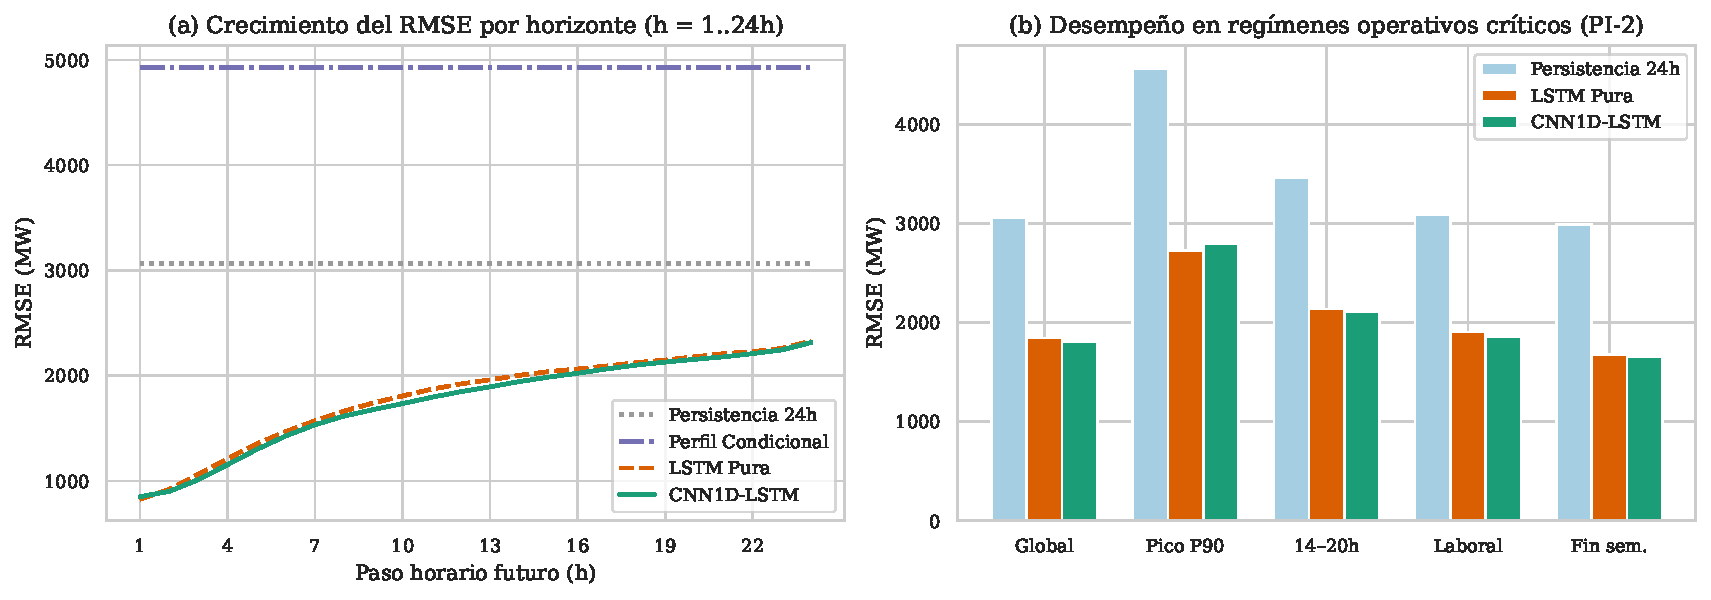
\includegraphics[width=0.88\textwidth]{figures/fig5_horizon_and_regimes.pdf}
    \caption{Diagnóstico desagregado (PI-2): (a) degradación del RMSE a lo largo de las 24 horas futuras; (b) comparación de RMSE por régimen operativo crítico.}
    \label{fig:horizon_regimes}
\end{figure*}

\begin{table}[htbp]
\centering
\caption{Desempeño por Régimen Operativo en Validación (RMSE / MAPE)}
\label{tab:regimes}
\footnotesize
\begin{tabular}{l r c c}
\toprule
\textbf{Régimen Operativo} & \textbf{Puntos} & \textbf{LSTM Pura} & \textbf{CNN1D-LSTM} \\
\midrule
Global & 517{,}080 & $1{,}845.75$ / $4.29\%$ & $\mathbf{1{,}806.45}$ / $\mathbf{4.12\%}$ \\
Franja Pico ($14\text{--}20\,\text{h}$) & 150{,}815 & $2{,}138.31$ / $4.54\%$ & $\mathbf{2{,}108.24}$ / $\mathbf{4.39\%}$ \\
Valle de Demanda ($<P_{90}$) & 475{,}575 & $1{,}747.63$ / $4.26\%$ & $\mathbf{1{,}692.04}$ / $\mathbf{4.05\%}$ \\
Días Laborales & 369{,}596 & $1{,}907.66$ / $4.27\%$ & $\mathbf{1{,}861.49}$ / $\mathbf{4.08\%}$ \\
Fines de Semana & 147{,}484 & $1{,}680.61$ / $4.34\%$ & $\mathbf{1{,}660.51}$ / $\mathbf{4.22\%}$ \\
Pico Extremo ($\ge P_{90}$) & 41{,}505 & $\mathbf{2{,}728.90}$ / $\mathbf{4.69\%}$ & $2{,}801.73$ / $4.85\%$ \\
\bottomrule
\end{tabular}
\end{table}

\section{Discusión Preliminar y Plan Ajustado}

\subsection{Interpretación Crítica y Dificultades Encontradas}
Los resultados preliminares confirman parcialmente nuestras hipótesis y revelan desafíos metodológicos clave:
\begin{enumerate}
    \item \textbf{Suavizado convolucional en extremos ($\ge P_{90}$):} Aunque los filtros CNN-1D reducen el error global, el ruido en valles y la latencia de inferencia, el operador \texttt{MaxPool1D(2)} combinado con \texttt{Dropout1d(0.2)} atenúa ligeramente la amplitud en el 10\,\% de horas de demanda extrema ($2{,}801.7$ vs.\ $2{,}728.9$\,MW), donde las variaciones obedecen a extremos térmicos rápidos.
    \item \textbf{Ausencia de variables meteorológicas exógenas:} Como evidencia el 17--19 de junio en la Fig.~\ref{fig:forecasts}(a), un modelo entrenado únicamente con demanda histórica y variables calendario posee un techo físico de predictibilidad cuando ocurren olas de calor o descensos bruscos de temperatura no reflejados en la historia reciente \cite{lim2021time,ahajjam2022experimental}.
    \item \textbf{Varianza entre semillas vs.\ margen de mejora:} En validación completa, la ganancia media de CNN1D-LSTM sobre LSTM Pura ($38.4$\,MW) es comparable a la desviación estándar entre semillas ($33.7\text{--}38.4$\,MW), y las semillas exhibieron paradas tempranas heterogéneas (época 21 en \texttt{pure\_lstm} \texttt{seed=42} vs.\ 50 en \texttt{seed=123}). Esto impide aún declarar superioridad estadísticamente concluyente antes de sintonizar hiperparámetros y aplicar pruebas formales de Diebold-Mariano \cite{diebold1995comparing}.
    \item \textbf{Limitación de escalabilidad de SARIMA:} Ajustar SARIMA$(1,1,1)\times(1,1,1)_{24}$ requirió $\sim 10.1$\,s por ventana de 60 días; evaluarlo exhaustivamente sobre las $21{,}545$ ventanas demandaría $\sim 60$ horas de CPU, lo que justifica su evaluación estratificada y evidencia la ventaja operativa de las redes neuronales ($0.013$\,ms/ventana).
    \item \textbf{Lecciones en pruebas y diagnóstico:} Durante la depuración inicial se corrigieron dos fallos documentados: (i) series sintéticas demasiado cortas en tests unitarios tras aislar los splits con \texttt{lag\_168}, y (ii) el cálculo de diferenciación estacional en ADF ($y_t - y_{t-24}$ en lugar de diferencias de orden 24 que causaban colinealidad numérica).
\end{enumerate}

\subsection{Plan de Trabajo Ajustado (Semanas 11 a 15)}
A partir de los hallazgos obtenidos, la Tabla~\ref{tab:plan_ajustado} detalla el cronograma depurado hacia el Entregable 3.

\begin{table}[htbp]
\centering
\caption{Plan Ajustado para las Últimas 5 Semanas (Hacia Entregable 3)}
\label{tab:plan_ajustado}
\footnotesize
\begin{tabularx}{\columnwidth}{c l p{3.8cm} l}
\toprule
\textbf{Sem.} & \textbf{Fase} & \textbf{Actividades Específicas} & \textbf{Resp.} \\
\midrule
11 & Optimización & Búsqueda bayesiana con Optuna \cite{akiba2019optuna} sobre \texttt{val} (tasa de aprendizaje, filtros, \textit{dropout}, ventana $W \in \{72, 168\}$). & A.\ Mosquera \\
12 & Ablación & Ablación estructural en \texttt{val}: sin \texttt{MaxPool1D}, $\pm$\texttt{Dropout1d}, variante CNN-GRU \cite{sajjad2020novel} y TCN \cite{bai2018empirical}. & A.\ Mosquera / J.\ Villalba \\
13 & Evaluación Ciega & Liberación única del split \texttt{test} (2016--2018), pruebas de significancia Diebold-Mariano \cite{diebold1995comparing} y errores por estación. & S.\ Cadena \\
14 & Consolidación & Discusión crítica, amenazas a la validez, ética de datos y figuras finales. & Equipo \\
15 & Entrega 3 & Artículo IMRaD completo (8--12 págs.) y repositorio final documentado. & Equipo \\
\bottomrule
\end{tabularx}
\end{table}

\section{Declaración de Integridad Académica}
En cumplimiento de los lineamientos del curso, se declara explícitamente que se emplearon herramientas de inteligencia artificial generativa como asistencia instrumental en: (1) refactorización modular y depuración sintáctica de scripts en PyTorch y pruebas \texttt{pytest}; (2) validación bibliográfica cruzada de metadatos DOI respecto al entregable previo; y (3) soporte de redacción técnica y maquetación en \LaTeX. La concepción experimental, la ejecución sobre los datos reales PJME en GPU, la interpretación crítica de resultados y el control de versiones en GitHub (\url{https://github.com/AnthonnyM31/Proyecto-IA-2-Parte-2}) son responsabilidad íntegra de los autores.

\bibliographystyle{IEEEtran}
\bibliography{referencias}

\end{document}
